\section{Design dimensions}\label{sec:designdims}

Language designers must decide how the async/await syntax will expand into the set of asynchronous building blocks. The expansion is often influenced by patterns in the pre-existing base language as well as performance and memory expectations of the community.

In this section we provide the async/await design dimensions. The design dimensions map the async/await syntax to the runtime behavior of the desugared program. The design dimensions are: \textit{eagnerness,} \textit{extent,} \textit{reference strength,} \textit{destruction,} \textit{propagation,} \textit{suspension,} and \textit{cancellation.}

\subsection{Eagerness}\label{ssec:designdims:eagerness} The Eagerness axis defines the eagerness of an async function application, the possible values are: \textit{eager,} \textit{semi-eager,} and \textit{lazy.}

On evaluating an eager async application, the current thread transfers execution to the body of the async function. When a suspension occurs, the application evaluates to a \task value and execution of the calling context proceeds as normal. By contrast, a \textit{semi-}eager application evaluates immediately to a \task value, but control does not transfer to the function body. The \task is scheduled with the executor to run on the next available worker thread. A lazy application evaluates immediately to a \coro object. As you may recall, \coros are not scheduled with the evaluator and perform work only when prompted.

\begin{figure}[H]
  \raggedright
  \begin{minipage}[t]{0.30\textwidth}
\begin{lstlisting}[language=Rust]
async fn work(msg: &str) {
  sleep(one_ms).await
  print!("{msg}");
}

#[tokio::main]
async fn main() {
  let a = work("A");
  let b = work("B");
  print!("C");
  a.await; b.await;
} // => CAB
\end{lstlisting}
    \cprotect\subcaption{Rust function applications are lazy. The function \code{work} does not execute until line eleven. The print order of the program is always ``CAB'' because \code{a}, and \code{b} are not running concurrently.}
    \label{fig:designdims:eagerness:lazy}
  \end{minipage}\hfill%
  \begin{minipage}[t]{0.33\textwidth}
\begin{lstlisting}[language=Swift]
func work(msg: String
) async throws {
  try await Task.sleep(
    for: .milliseconds(1))
  print(msg)
}

async let a = work(msg: "A")
async let b = work(msg: "B")
print("C")
try await a; try await b
// => CAB, CBA, BCA, ACB, ...
\end{lstlisting}
    \cprotect\subcaption{Swift function applications are semi-eager. The right-hand-side of an async let binding is evaluated in a concurrently executing \textit{child} task, control of the executing task does not jump to the body of the async function. The print order of the program is any permutation of the string ``ABC''.}
    \label{fig:designdims:eagerness:semieager}
  \end{minipage}\hfill%
  \begin{minipage}[t]{0.33\textwidth}
\begin{lstlisting}[language=CSharp]
async Task work(string msg) {
  Console.Write(msg);
  await Task.Delay(1);
}

async Task Main() {
  var a = work("A");
  var b = work("B");
  Console.Write("C");
  await a; await b;
} // => ABC
\end{lstlisting}
    \cprotect\subcaption{\CSharp{} function applications are eager. In this example the order of statements in the \code{work} function are flipped, the print happens before the delay. When \code{work} is called the executing thread transfers control to the body of the async function until it is suspended. The print order of this program is always ``ABC''.}
    \label{fig:designdims:eagerness:eager}
  \end{minipage}
  \caption{Examles of lazy, semi-eager, and eager async function application.}
  \label{fig:designdims:eagerness}
\end{figure}

Languages have adopted all variants of eagerness, as shown in \Cref{fig:designdims:eagerness}. Rust employes lazy function evaluation, \coro values perform work only when awaited, polled, or spawned. \Cref{fig:designdims:eagerness:lazy} shows work being performed at an await point, resulting in a deterministic order of effects.

Swift's \textit{async let} construct is semi-eager, as shown in \Cref{fig:designdims:eagerness:semieager}, the right-hand-side of the binding is scheduled to run in a concurrently executing child task. Note that in Swift async applications, which are not immediately awaited, must be bound with an \textit{async let} instead of a normal let binding. The order of effects in this program is non-deterministic.

\CSharp adopts a truly eager application, the currently executing thread will transfer execution to the body of the async function. In \Cref{fig:designdims:eagerness:eager}, the order of the print and delay statements are flipped in the body of the \code{work} function. Because applications are eagerly evaluated, the order of effects is deterministic.

The choice of eagnerness is a tradfeoff in predictability, maximizing \abbr{cpu} utilization, and optimizing for fast paths. Lazy evaluation has three main benefits. First, lazy evaluation can provide predictable memory allocation. Asynchronous function applications evaluate directly to a \bum value that can be stack allocated. If the \bum needs to run in parallel or be stored on the heap, the developer must explicitly make this operation. Predictable memory allocation is one main motivation for Rust's async/await design~\cite{withoutboats_why_2023}. Second, lazy evaluation provides predictable performance and effect orderings. In lazily-evaluated async/await, developers compose computations using declarative functions and then run the staged computation when its value is awaited. Developers explicitly state when two computations can proceed concurrently and how errors (e.g., raised exceptions) from one affect concurrently running computation --- for example, the \code{join!} vs \code{try_join!} operator in Tokio (Rust). Third, lazily-evaluated languages that \bum values can provide the Executor and Reactor as user-space libraries, instead of shipping them bundled in the language runtime. Communities can then provide their own asynchronous runtime that is tailored towards a specific need when a preexisting runtime is insufficient.

Semi-eager evaluation maximizes \abbr{cpu} utilization while protecting the calling thread. Protecting the current thread is important for responsiveness in App/UI development, such as in the SwiftUI framework.

Eager evaluation is beneficial to optimize the fast paths in synchronous-executing functions. Asynchronous functions \textit{may} perform asynchronous operations, but many do not. For example, a function that performs network \abbr{io} may want to buffer data so that subsequent calls execute synchronously; they simply read from the buffer and do not go to the network. Eagerly-evaluating systems can avoid the runtime and memory overhead of asynchronous function calls when the calls terminate synchronously.


\subsubsection{\Extent}\label{ssec:designdims:extent}

\begin{figure}[t]
  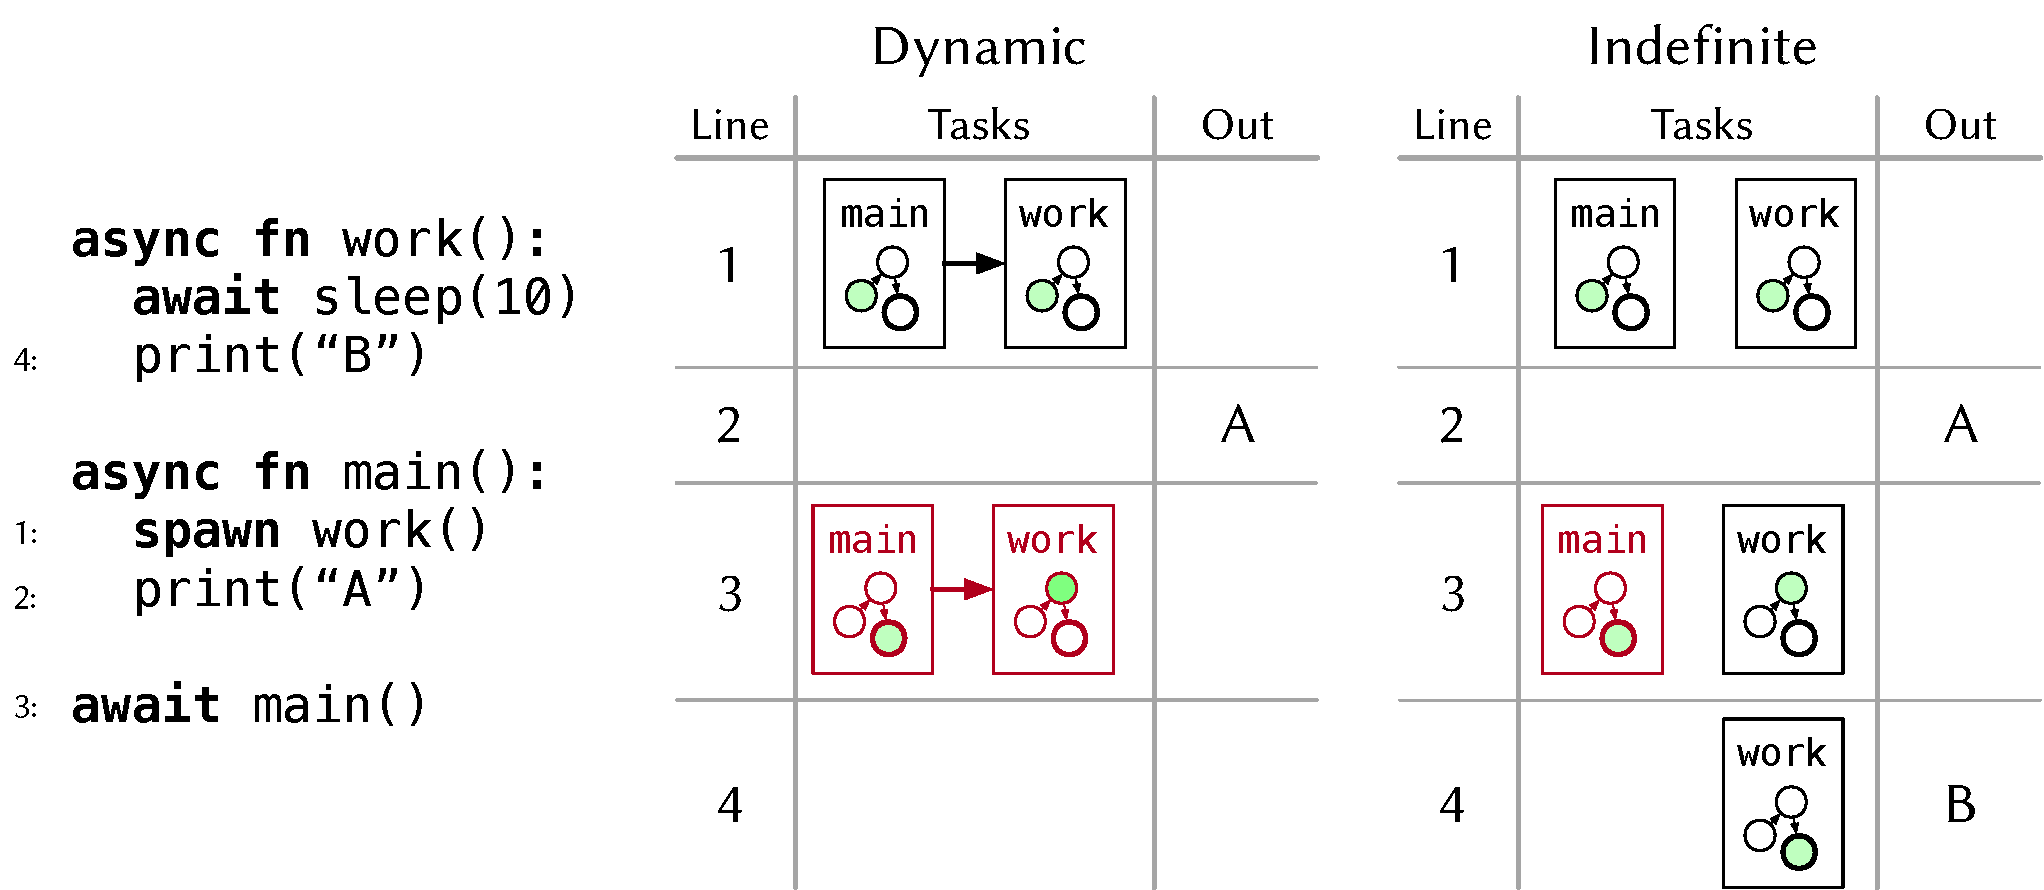
\includegraphics[width=0.82\linewidth]{./f/extent.pdf}
  \caption{An example program demonstrating the \extent dimension, executed with Swift (\dyn) and \Js (\indef). Each column shows the task structure and output after executing each line. Arrows between tasks indicate a parent-child relationship used for \dyn \extent.}
  \label{fig:extent}
\end{figure}

% \begin{figure}[t]
%   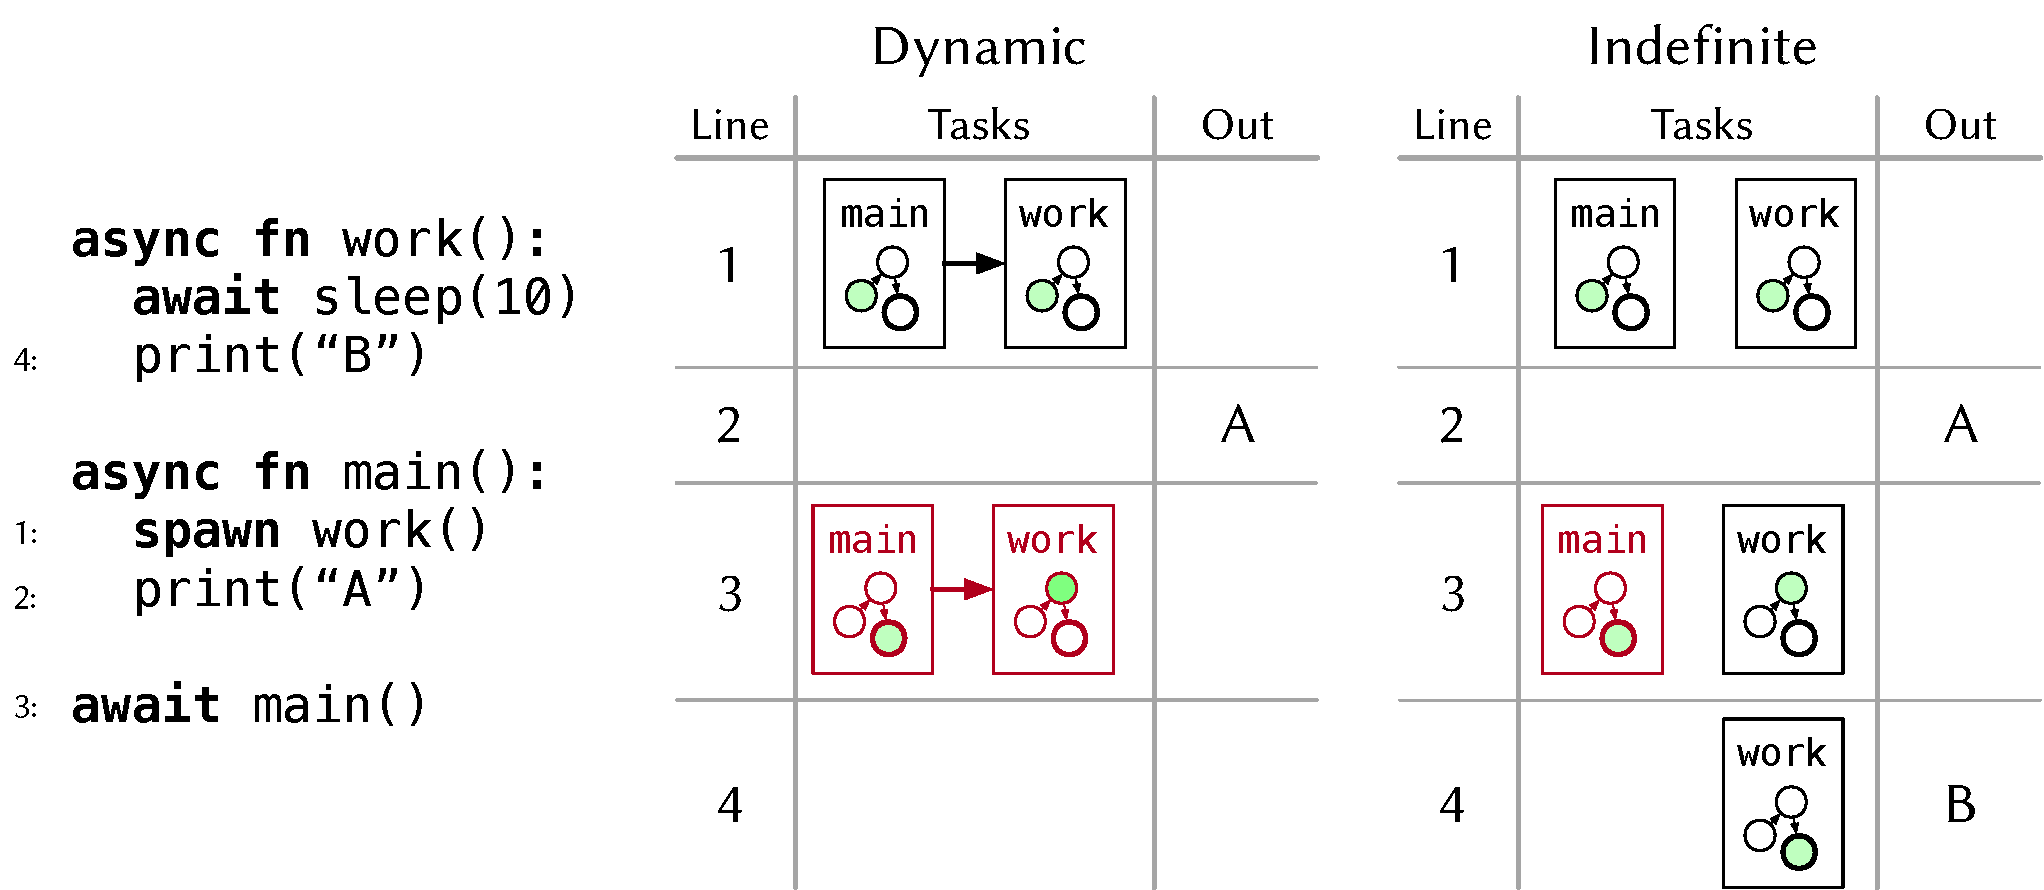
\includegraphics[width=0.7\linewidth]{./f/extent.pdf}
%   \caption{An example program demonstrating the \extent dimension, executed with Swift (\dyn) and \Js (\indef). Each column shows the task structure and output after executing each line. Arrows between tasks indicate a parent-child relationship used for \dyn \extent.}
%   \label{fig:extent}
% \end{figure}

Borrowing terminology from the Lisp community, the \extent of a task is the interval of time during which that task is capable of executing. For example, consider the program in \Cref{fig:extent}. What is the extent of the \code|spawn child_work()| task? The answer is it depends on quite a number of factors, as previously illustrated in \Cref{fig:motivating-example}.

In some designs for straight-line asynchrony, especially earlier designs, tasks by default have an \indef \extent: the task can live until it is no longer reachable, at which point the task is destructed. \Js, \CSharp, Python+Asyncio, and Rust+Tokio/Smol all use \indef \extent. Note that designs differ on how to determine reachability (see \Cref{ssec:designdims:references}), and designs also differ on the mechanism for destruction (see \Cref{ssec:designdims:destruction}). \Cref{fig:extent} illustrates \indef \extent, showing how the \code|child_work()| task outlives its parent \code|parent_work()| task, and the program waits until the work is completed.

Some have called \indef \extent an ``unstructured'' approach to asynchrony~\cite{smith_thoughts_2016}, akin to using goto for control flow, as task handles can easily go unhandled, leaving asynchronous work dangling with no clear policy for managing it.
%
This line of thought has led to the devleopment of ``structured'' asynchrony approaches~\cite{sustrik_structured_2025,mccall_swift_2021,elizarov_kotlin_2021}, which we describe as having \dyn \extent, found in Swift and Python+Trio. With \dyn \extent, a task's extent is tied to the extent of another task. In \Cref{fig:extent}, under \dyn \extent, the \code|child_work()| task is associated with the \code|parent_work()| task. When the \code|parent_work()| task completes, its associated tasks are destructed, which means cancellation in the case of Swift. Therefore the second print never occurs.

\paragraph{Design rationale.}

The main argument for \dyn \extent is that limiting tasks to known scopes leads to programs that are easier to reason about, and compose better with other language features~\cite{mccall_swift_2021,elizarov_kotlin_2021}. For instance in Python, \dyn \extent can ensure that a task within a \code|with| block will not use resources (e.g., file descriptors) after they have been cleaned up~\cite{smith_thoughts_2016}. However, existing implementations of \dyn \extent only support a strictly hierarchical model of parent-child task relationships (via \code|TaskGroup| in Swift and \code|Nursery| in Trio). These implementations disallow programs that might have more complex dependencies between tasks, such as two parent tasks awaiting the same child task.


\subsection{Reference Strength}\label{ssec:designdims:references}

The Runtime Reference Strength axis defines the strength of \task references held by the runtime. The possible values are: \textit{strong,} and \textit{weak.}

\begin{figure}[H]
  \begin{subfigure}[t]{0.49\textwidth}
\begin{lstlisting}[language=Rust]
use std::time::Duration;
use smol::Timer;
const sleep: fn(Duration) -> Timer =
  Timer::after;

async fn heartbeat() {
  loop {
    sleep(Duration::from_millis(1)).await;
    print!(".")
  }
}

async fn work() {
  let t = smol::spawn(heartbeat());
  sleep(Duration::from_millis(5)).await;
  print!("A");
}

fn main() {
  smol::block_on(async {
    work().await;
    print!("B");
    sleep(Duration::from_millis(5)).await;
  })
} // => "....AB"
\end{lstlisting}
    \cprotect\caption{An  example of  weak  runtime references. The SMOL (Rust) framework does not hold strong references to running \tasks. The program prints ``....AB'' with never any trailing periods after the `B.'}
    \label{fig:designdims:refs:weak}
  \end{subfigure}\hfill%
  \begin{subfigure}[t]{0.49\textwidth}
\begin{lstlisting}[language=Rust]
use std::time::Duration;
use tokio::time::sleep;



async fn heartbeat() {
  loop {
    sleep(Duration::from_millis(1)).await;
    print!(".")
  }
}

async fn work() {
  let t = tokio::spawn(heartbeat());
  sleep(Duration::from_millis(5)).await;
  print!("A");
}

#[tokio::main]
async fn main() {
  work().await;
  print!("B");
  sleep(Duration::from_millis(5)).await;
} // => "....AB...."
\end{lstlisting}
\cprotect\caption{An  example of  strong  runtime references. The Tokio (Rust) framework holds strong references to running \tasks. The program prints ``....AB....'' with some amount of trailing periods printed during the sleep within the \code{main} function.}
    \label{fig:designdims:refs:strong}
  \end{subfigure}
  \cprotect\caption{An example of weak and strong runtime references.}
  \label{fig:designdims:refs}
\end{figure}

The \task reference strength held by the runtime is important for systems with \textit{indefinite} \task extent (see \Cref{ssec:dims:extent}). Shown in \Cref{fig:designdims:refs:weak} the SMOL (Rust) system holds weak pointers to running \tasks.\footnote{The \code{.detach()} method can be invoked on \tasks to transfer ownership to the runtime system, turning the default weak references into strong references.} When no more references exist to the \task \code{t}, established on line 14, the \task is cancelled and deallocated. The output will have no trailing periods printed  because the heartbeat task is cancelled on line 17 when the reference \code{t} goes out of scope.

In contrast, the Tokio (Rust) system holds strong references to \tasks. The \task referenced by \code{t} is not destroyed when \code{t} goes out of scope, because the runtime continues to hold a reference to the \task. The output will contain some number of trailing periods after the `B,' as the heartbeat \task continues to execute while the main function sleeps on line 23.

Weak runtime references are used by SMOL (Rust) to prevent dangling \tasks from consuming resources without the devlopers knowledge. A \task is automatically cancelled and deallocated when no further references to it exist; a deterministic effect thanks to Rusts ownership type system. This behavior parallels the behavior of memory allocation in Rust. Asyncio (Python) also holds weak references to \tasks, which is a source of controversy in the ecosystem~\cite{hartl_asyncio_2022}. At the time of writing, Asyncio's use of weak references is marked as a bug, however, the community is hesitant to change the design without understanding why it was designed this way to begin with; a fact that is undocumented and not remembered by the core developers.


\subsubsection{\Destruction}\label{ssec:designdims:destruction} 

\begin{figure}[t]
  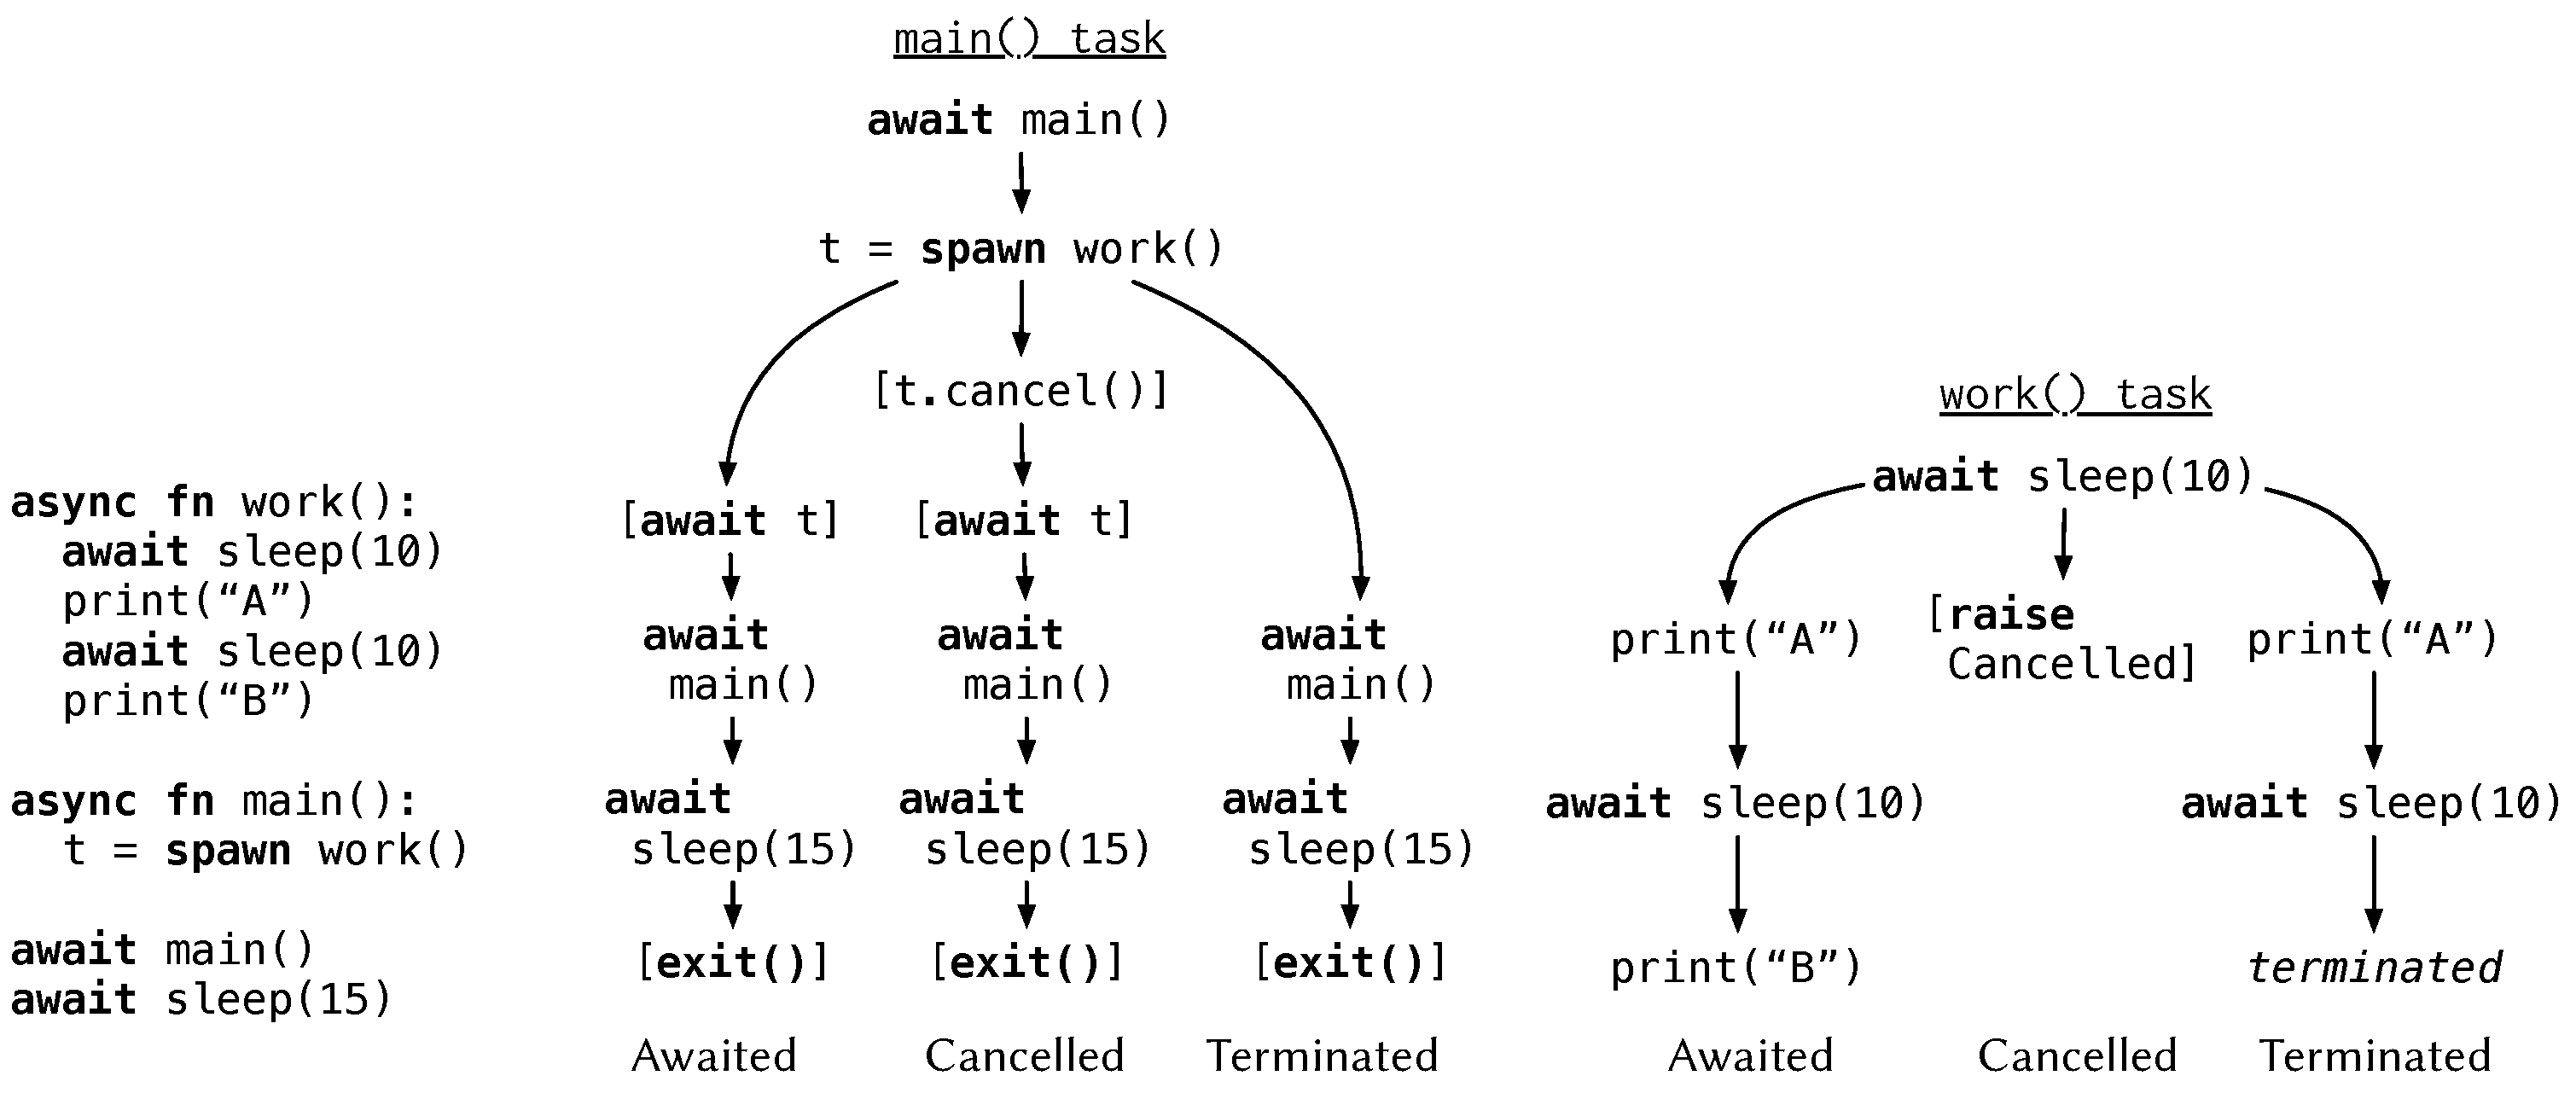
\includegraphics[width=\linewidth]{f/destruction.pdf}
  \caption{\Destruction [CAPTION TODO]}
  \label{fig:destruction}
\end{figure}


Once a language has decided that it is time to destruct a task, we encounter yet another point of divergence: what does it mean to destruct a task? For example, consider the program in \Cref{fig:destruction}. At the end of the \extent of the spawned \lstinline[language=Pseudo]|work()| task (either end of \lstinline[language=Pseudo]|main()| for \dyn \extent, or end of program for \indef \extent), what happens to the \lstinline[language=Pseudo]|work()| task? Today's languages offer three possibilities: to \emph{await} the task, to \emph{cancel} the task, and to \emph{terminate} the task.

The \destruction dimension is orthogonal to \extent. \Js is a language with \indef \extent and awaiting destruction --- \Cref{fig:extent} previously showed an example relying on this pair of design decisions. Python+Trio is a language/system with \dyn \extent and awaiting destruction, as tasks are tied to a ``nursery,'' and the nursery waits until all its child tasks are completed before exiting. The awaiting column in \Cref{fig:destruction} demonstrates Trio semantics, where the program would print ``ABC'' by waiting for the \lstinline[language=Pseudo]|work()| task to before exiting \lstinline[language=Pseudo]|main()|.

Most other designs opt to cancel tasks at the end of extent, such as Swift, Rust+Tokio, Rust+Smol, and Python+Asyncio. [TODO: ARE SMOL AND SWIFT ACTUALLY COMPARABLE?]


% The \Task Destruction axis defines what happens to a task when the \task object is destroyed by the system. The possible values are: \textit{awaited,} \textit{cancelled,} or \textit{terminated.}

% \Cref{fig:designdims:destruction:await} shows an example JavaScript program that awaits \tasks on destruction~\missingcite, even though there is no explicit \code{await} keyword. The program terminates after 10 seconds and prints ``exiting'' and ``done.''

% \Cref{fig:designdims:destruction:cancel} shows an example Swift program that cancels a running task on destruction~\missingcite. Because that task is executing a long sleep operation, the sleep is cancelled --- on cancellation \code{Task.sleep} raises an exception that we suppress with the \code{try?} keyword --- and the program continues executing. The program terminates after ~0.5 seconds and prints ``exiting,'' ``cancelled'' and ``done.''

% \Cref{fig:designdims:destruction:term} shows an example \CSharp program that terminates running \tasks on destruction~\missingcite. The program terminates after ~0.5 seconds and prints ``exiting.''

% Where your language falls on the destruction axis informs the safety and responsiveness of the system. Await destruction allows running \tasks to complete, which provides data/invariant integrity for the program at the expense of responsiveness.

% Cancel destruction may provide \tasks the chance to safely reclaim resources --- depending on the language's chosen cancellation semantics --- however, programs may still suffer from responsiveness issues if cancelling a \task requires the \task's cooperation. We discuss cancellation semantics in \Cref{ssec:designdims:cancellation}.

% Terminate destruction prioritizes speed over safety. A running \task may hold system resources or be in the middle of an operation, by cancelling the \task the system risks deadlocks and breaking logical invariants.


\subsubsection{\Propagation}\label{ssec:designdims:propagation}

\begin{wrapfigure}{r}{0.37\linewidth}
\begin{lstlisting}[language=Py]
from trio import open_nursery

async def fail():
  raise Exception()

async def main():
  print("A")
  async with open_nursery() as n:
    n.start_soon(fail)
  print("B")
\end{lstlisting}
  \cprotect\caption{An example of \destruct \propagation. Python+Trio reraises exceptions when their associated nursery scope ends.}
  \label{fig:propagation:trio}
\end{wrapfigure}

One final point of divergence at a task's end of life is the handling of exceptions. In all surveyed languages with exceptions (Python, Swift, \Js, \CSharp), awaiting on an async function that has thrown an exception will re-raise the exception at the await point.\footnotemark{} However, what happens to an exception raised in a task that is never awaited? We call this the \propagation dimension.%
\cprotect\footnotetext{Instead of exceptions Rust uses the \code|Result| type to communicate errors. An \code|Err| variant is returned on await, which we consider a semantically equivalent design to re-raising an exception at the await point.}

Most languages \never propagate, meaning the exception generates no behavior outside its containing task, apart from perhaps printing to the console. Python+Asyncio and \Js will print a stack trace for an uncaught asynchronous exception. Node.js\ specifically will exit with a non-zero error code, although this latter behavior is not part of the ECMAScript specification so we still categorize it as a \never approach to \propagation.

Python+Trio is the only system which offers a different semantics, in part because tasks cannot be awaited, so the library must offer another mechanism for observing asynchronous exceptions. The example in \Cref{fig:propagation:trio} (shown in Python, not pseudocode) will print ``A'' but not ``B'' because the nursery will re-raise the exception originating in the \code|fail| function. We describe this as \destruct \propagation. A similar program in any other system will print ``A'' then ``B'', possibly with a stack trace printed in-between.

\paragraph{Design rationale.} The upside to the \destruct approach is that an application is less likely to ignore problematic exceptions. With the \never approach, if a developer does not carefully monitor their logs, a task can fail and cause confusing bugs where expected operations never occur. 

The downside is that the \destruct approach may run counter to either a developer's intuitions (i.e., exceptions aren't thrown away by the system) or their desired software architecture. Concurrency \abbr{api}s often seek to encapsulate errors at thread or task boundaries, so errors in one thread cannot crash the whole system. For example, in a backend web server with many concurrent connections, it is likely undesirable that one exceptional connection should crash the entire server. Either way, it seems sensible that that a straight-line asynchrony \abbr{api} should offer \emph{some} way of accessing information about unawaited exceptions, rather than only printing to standard error, or ignoring unawaited exceptions outright.


\subsubsection{\Suspension}\label{ssec:designdims:suspension}

\begin{figure}[t]
  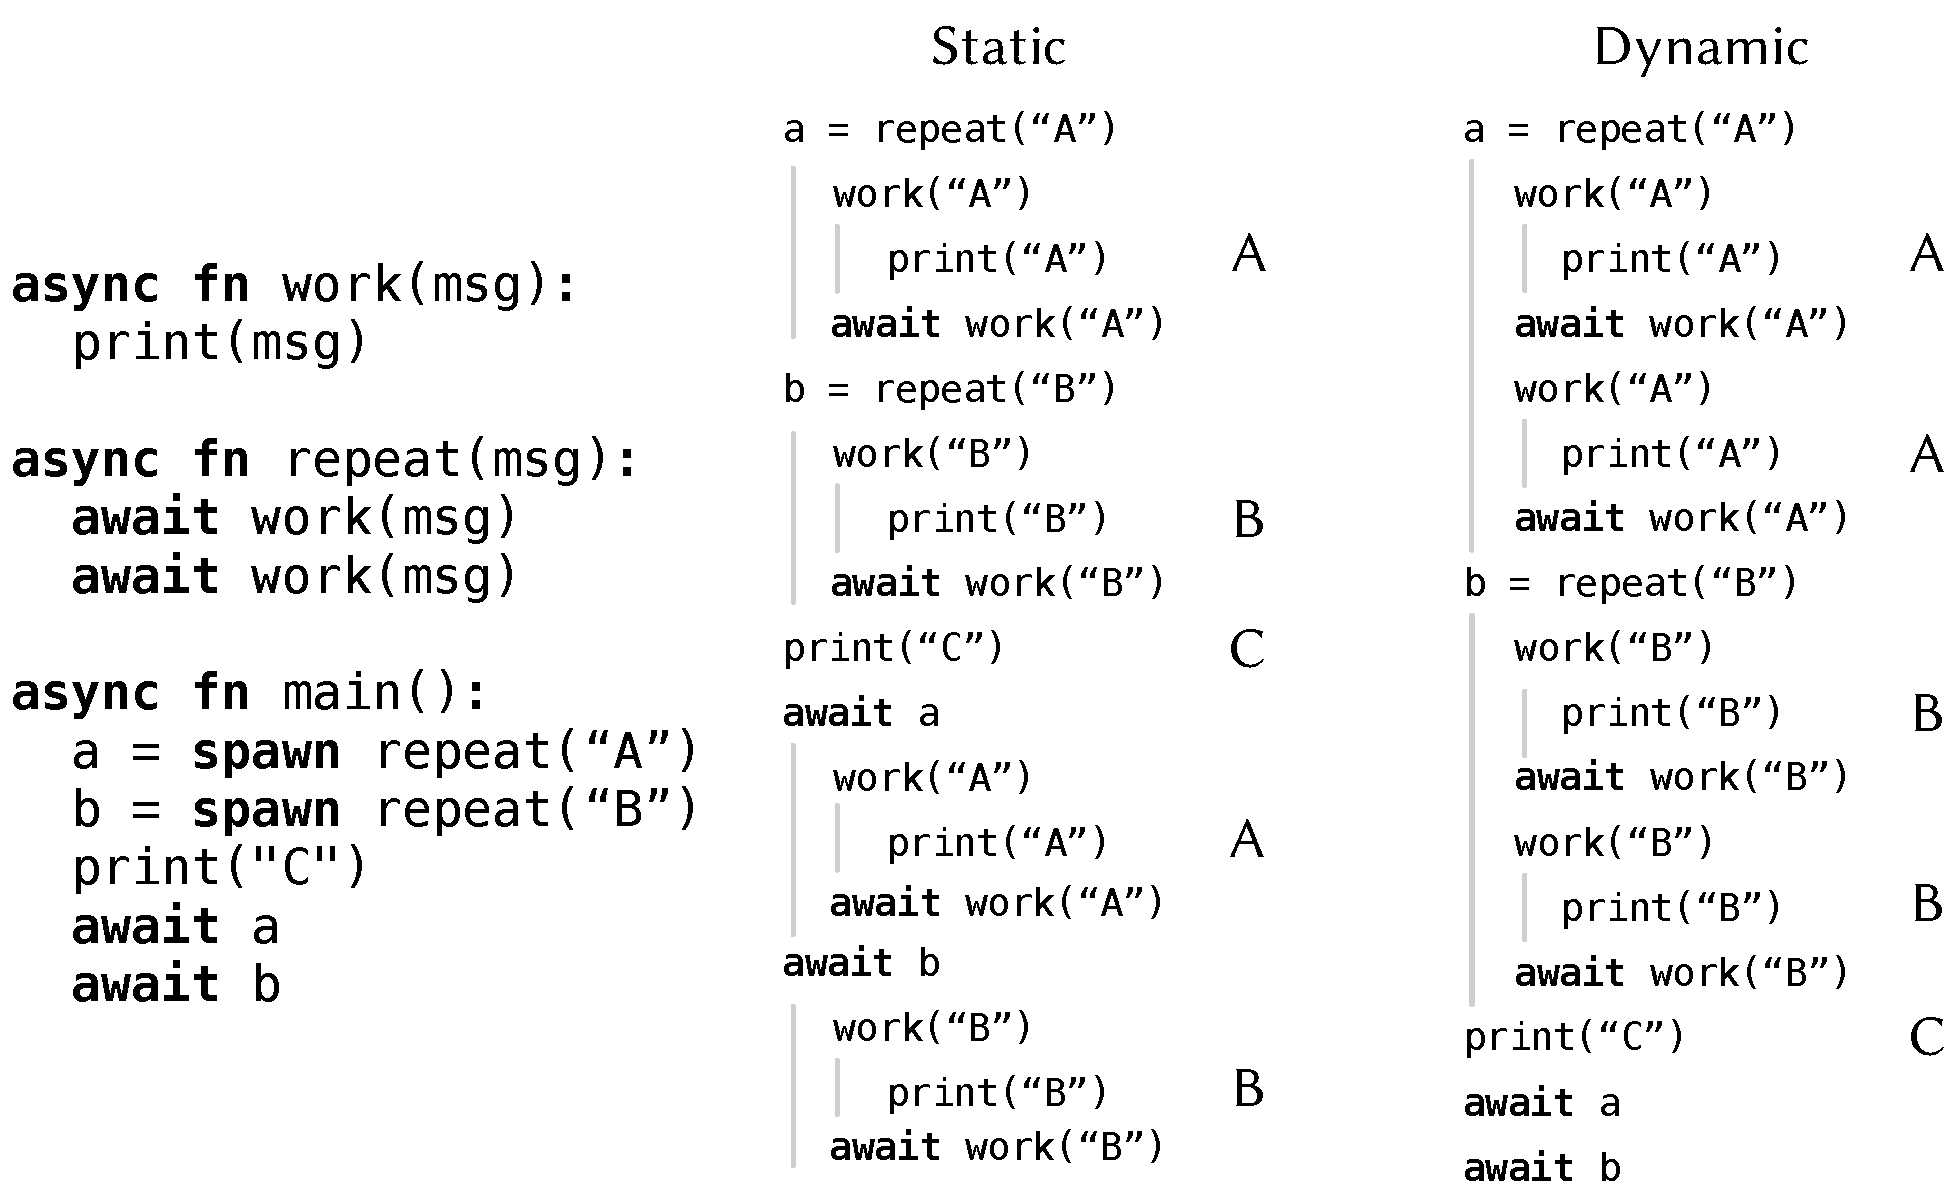
\includegraphics[width=0.7\linewidth]{f/suspension.pdf}
  \caption{An example program demonstrating the \Suspension dimension, executed with \Js (\static) and \CSharp (\dynamic). Each column shows an execution trace of the program under an eager semantics with each kind of \suspension. The execution traces are nested according to their level in the call stack, and the order of prints to stdout is emphasized in the right part of each column.}
  \label{fig:suspension}
\end{figure}

Once asynchronous work has started, the next design divergence occurs at await points. The \Suspension dimension defines the guarantees a language makes about whether an await point is guaranteed to yield control. For example, consider the program in \Cref{fig:suspension} executing under an \eager semantics. The line \code|a = repeat("A")| will call into \code|work("A")| which will call \code|print("A")| and return to \lstinline[language=Pseudo]|await work("A")|. The task for \code|work("A")| has been completed, so a language has two choices: either yield control to the caller, or continue evaluation past the \lstinline[language=Pseudo]|await|. We call the former strategy \emph{\static} suspension because an await point is statically guaranteed to always yield. We call the latter strategy \emph{\dynamic} suspension because whether an await point yields depends on the awaited task.

In only one language surveyed, \Js, an await point is guaranteed to yield according to the ECMAScript specification \cite[\textsection 27.7.5.3, step 3.b]{ecma_ecmascript_nodate}. Therefore in \Cref{fig:suspension}, running under \Js semantics, the program outputs ``ABCAB'' because \lstinline[language=Pseudo]|await work("A")| yields back to \code|main|. In all other languages, no such guarantee exists. For the example program operating under an eager semantics such as in \CSharp, the program would output ``AABBC'' because \lstinline[language=Pseudo]|await work("A")| observes that \code|work("A")| is complete and therefore the await expression can continue evaluation.

\paragraph{Design rationale.}

The principal reason to adopt \static suspension is to prevent starvation. Under an eager approach with \dynamic suspension, if a compute-bound task is called before calling \abbr{i/o}-bound tasks, the first task can starve the remaining tasks of CPU time. A \static suspension policy reduces the likelihood of that compute-bound task never yielding control back to the executor.

\Static suspension comes at a performance cost. In the case of awaiting a completed task, \static suspension requires a round-trip to the runtime and back to continue past the await. Languages with \dynamic suspension can mitigate the starvation issue by providing a \code|yield_now| primitive which has no effect but to yield control to the runtime.



\subsubsection{Cancellation} The Cancellation axis defines how a running task is cancelled, including how cancellation is signaled, if at all, and how cancellation propagates between task dependencies. A clear cancellation mechanism is what distinguishes async/await from other concurrency paradigms. Within the cancellation axis there are two design dimensions: \textit{cooperation,} and \textit{direction.}

\ggnote{This section has not been updated}

In this section we will illustrate cancellation using the function \code{process} defined in \Cref{fig:cancellation} in both Rust (SMOL) and Python (AsyncIO).

\begin{figure}
  \begin{minipage}[t]{0.49\textwidth}
\begin{lstlisting}[language=Rust, linebackgroundcolor={\lineEq{15}}]
async fn process(
  db: Database,
  cache: Cache,
  request: Request,
) -> Response {
  let response = compute_response(
    &db, &cache, request).await;

  let db_update = smol::spawn(
    update_db(&db, &response));

  let cache_update = smol::spawn(
    update_cache(&cache, &response));

    db_update.await;
    cache_update.await;

  response
}
  \end{lstlisting}
  \end{minipage}\hfill%
  \begin{minipage}[t]{0.49\textwidth}
\begin{lstlisting}[language=Python, linebackgroundcolor={\lineEq{11}}]
async def process(db, cache, request):
  response = await compute_response(
    db, cache, request)

  db_update = asyncio.create_task(
    update_db(db, response))

  cache_update = asyncio.create_task(
    update_cache(cache, response))

  await db_update
  await cache_update

  return response
\end{lstlisting}
  \end{minipage}
  \cprotect\caption{An illustrative async function, \code{process}, that processes a request, and in turn, updates a database and cache in parallel. It's important that the cache and database remain in sync, but the chosen cancellation policy may break this invariant. (Left) A Rust implementation using the SMOL async framework. SMOL uses a top-down, non-cooperative cancellation policy that may leave the database and cache in a \textit{partially-updated} state. (Right) A Python implementation using the Asyncio library. Asyncio uses a bottom-up, cooperative cancellation policy that may leave the database unchanged and the cache fully updated.}
  \label{fig:cancellation}
\end{figure}

\paragraph{Cooperation} The Cooperation cancellation axis defines if cancellation requires cooperation from all tasks in the cancelled subtree. If cancellation is \textit{cooperative,} this means that a cancellation signal can get intercepted by a node in the tree if they do not cooperate. Cancellation is \textit{non-}cooperative if tasks have no choice but to cooperate with cancellation; non-cooperative cancellation can otherwise be referred to as termination.

In Rust a \Coro{} is represented as an enumeration. Cancelling an \Coro{} is defined by simply freeing the value's memory. In the asynchronous framework SMOL, a \Task{} can be cancelled by either invoking the \code{.cancel()} method or freeing the \Task{}, which in turn frees the underlying \Coro{}. As a consequence of Rust's choice to define cancellation as a memory free, it is not possible for an asynchronous function to prevent a cancellation. A memory free cannot be shielded or intercepted. Therefore, we classify Rust's cancellation as non-cooperative. Note that this cancellation policy remains non-cooperative regardless of the async framework chosen for a specific program.

\begin{figure}
  \begin{minipage}[t]{0.49\linewidth}
    \includegraphics[width=0.99\textwidth]{example-image-a}
  \end{minipage}\hfill%
  \begin{minipage}[t]{0.49\linewidth}
    \includegraphics[width=0.99\textwidth]{example-image-b}
  \end{minipage}
  \cprotect\caption{Example execution of the \code{process} function shown in \Cref{fig:cancellation}. (Left) The Rust (SMOL) implementation uses the non-cooperative memory free cancellation protocol. Both the \code{db_update} and \code{cache_udpate} are terminated, leaving the systems in a potentially inconsistent state. (Right) The Python (Asyncio) implementation uses exceptions to signal cancellation and the \code{cache_update} is left orphaned because cancellation is not signaled to it.}
  \label{fig:cancellation:swimlane}
\end{figure}

Shown in \Cref{fig:cancellation:swimlane}, if the executing Rust function \code{process} is cancelled at line fifteen, then the memory for \code{process}, \code{db_update}, and \code{cache_update} are all freed. Neither the database update nor the cache update can rollback partially-made changes, so unless both operations completed fully before the cancellation, the system is left in an inconsistent state.

Cancellation in Python is handled by raising an exception at the next await point blocking the task. Refering to the code in \Cref{fig:cancellation}, if the \code{process} function is cancelled at line eleven, the exception will be raised at an await point within the \code{update_db} function. Because \code{process} is waiting on \code{db_update}, an await point blocking the task is within the dynamic extent of \code{update_db}. The \textit{expectation} is that \code{update_db} will allow the exception to propagate, or reraise the exception if it needs to do some cleanup.

\begin{wrapfigure}{r}{0.35\textwidth}
  \raggedright
\begin{lstlisting}[language=Python,numbers=none]
async def db_update(db r):
  snap = await db.snapshot()
  try:
    # .. cancelled in here ..
  except:
    await db_rollback(snap)
\end{lstlisting}
  \cprotect\caption{An example of a Python function swalling a cancellation request. The function \code{db_update} is not cooperating in the cancellation protocol by using a try/except block, which catches all exceptions.}
  \label{fig:cancellation:cooperative}
\end{wrapfigure}

The \code{db_update} function may choose to, or be mistakenly programmed to, not cooperate with cancellation. \Cref{fig:cancellation:cooperative} provides an illustrative implementation of the \code{db_update} function that does not cooperate with the Asyncio cancellation protocol. A \code{asyncio.CancellationError} will get raised within the \code{db_update} function, however, since the function body is wrapped in a try/except block, the cancellation request is never propagated to the \code{process} function. \code{process} is unaware that the database was not updated and the database and cache are now out of sync.

\paragraph{Propagation direction} The Propagation Direction axis defines where in the waiting tree of dependencies cancellation is signaled first and how that signal is propagated to the rest of the waiting nodes. The possible values are \textit{top-down,} \textit{bottom-up,} and \textit{simultaneous.}

Before specifying exactly what the direction of cancellation propagation is, we first need to specify through what cancellation is propagating. Cancellation propagates through the \textit{task tree,} specifically, the task tree rooted at the cancelled task. Not all languages explicitly build a task tree in the runtime.

Consider the Rust (SMOL) code in \Cref{fig:cancellation}, at line fifteen, the set of tasks is depicted in \Cref{fig:cancellation:tree:rust}. Unlike Python, an edge between two tasks in the SMOL task tree is added when a task is \textit{spawned,} not when it's awaited. We say this because the calling task has ownership of the spawned task. When a task is cancelled, SMOL invokes the destructors as they would typically run in Rust, which flows down the tree represented by memory ownership. Therefore, we say that Rust (SMOL) cancellation propagates top-down.

\begin{wrapfigure}{l}{0.30\linewidth}
  {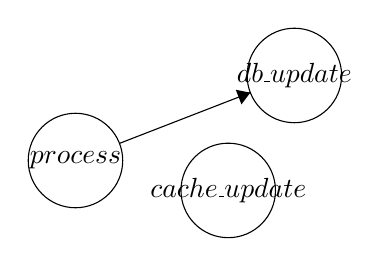
\begin{tikzpicture}[scale=0.2]
  \tikzstyle{every node}+=[inner sep=0pt]
    \draw [black] (13.3,-24.3) circle (3);
    \draw (13.3,-24.3) node {$\text{\tiny process}$};
    \draw [black] (27.2,-18.9) circle (3);
    \draw (27.2,-18.9) node {$\text{\tiny db\_update}$};
    \draw [black] (23,-26.2) circle (3);
    \draw (23,-26.2) node {$\text{\tiny cache\_update}$};
    \draw [black] (16.1,-23.21) -- (24.4,-19.99);
    \fill [black] (24.4,-19.99) -- (23.48,-19.81) -- (23.84,-20.74);
  \end{tikzpicture}
  \cprotect\subcaption{The state of the Python (Asyncio) task tree at line eleven. Because \code{process} is waiting on \code{db_update} the two form a tree, however, \code{cache_update} is not part of the current tree because it wasn't awaited.}
  \label{fig:cancellation:tree:python}}

  {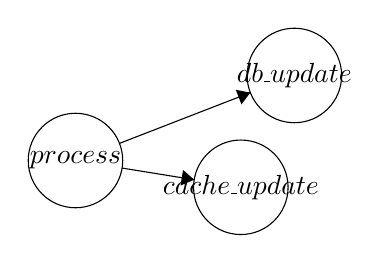
\begin{tikzpicture}[scale=0.2]
  \tikzstyle{every node}+=[inner sep=0pt]
  \draw [black] (13.3,-24.3) circle (3);
    \draw (13.3,-24.3) node {$\text{\tiny process}$};
  \draw [black] (27.2,-18.9) circle (3);
    \draw (27.2,-18.9) node {$\text{\tiny db\_update}$};
  \draw [black] (23.8,-26) circle (3);
    \draw (23.8,-26) node {$\text{\tiny cache\_update}$};
  \draw [black] (16.1,-23.21) -- (24.4,-19.99);
  \fill [black] (24.4,-19.99) -- (23.48,-19.81) -- (23.84,-20.74);
  \draw [black] (16.26,-24.78) -- (20.84,-25.52);
  \fill [black] (20.84,-25.52) -- (20.13,-24.9) -- (19.97,-25.89);
  \end{tikzpicture}
  \cprotect\subcaption{The state of the Rust (SMOL) task tree at line fifteen. Because SMOL's cancel on drop semantics, and Rust's owernship model, the task tree is help implicitly in Rust's memory.}
  \label{fig:cancellation:tree:rust}}

  \caption{The depicted task right before cancellation from the programs shown in \Cref{fig:cancellation}.}
  \label{fig:cancellation:tree}
\end{wrapfigure}

Consider the Python (Asyncio) code in \Cref{fig:cancellation}, at line 11, the set of tasks is depicted in \Cref{fig:cancellation:tree:python}. By default, all tasks in Asyncio are disjoint. Given two tasks, $A$ and $B$, where $B$ is spawned from within $A$, an edge in the task tree is added between the two nodes only when $A$ awaits $B$. Therefore, in our example program \code{db_update} is a child of \code{process} only because of the await present on line eleven. Therefore, cancellation is signalled from within \code{update_db}, and propagates \textit{upward} in the task tree to signal cancellation.

A \textit{simultaneous} cancellation would alert all tasks at the same time of cancellation. An example language with simultaneous cancellation propagation is Swift, as we will see in \Cref{sec:semantics}.



\subsection{Summary of Language Semantics}

\begin{table}
  \begin{tabular}{lllllll}
    \toprule
    System           & Eagerness   & Extent       & References   & Destruction  & Propagation  & Suspension  \\
    \midrule
    \CSharp          & eager       & indefinite   & strong  & terminated   & never        & dynamic     \\
    JavaScript       & eager       & indefinite   & strong  & awaited      & destruction  & static      \\
    Swift            & semi-eager  & dynamic      & -       & cancelled    & never        & dynamic     \\
    \midrule
    Tokio (Rust)     & lazy        & indefinite   & strong  & cancelled    & -            & dynamic     \\
    Smol (Rust)      & lazy        & indefinite   & weak    & cancelled    & -            & dynamic     \\
    \midrule
    AsyncIO (Python) & lazy        & indefinite   & weak    & terminated   & destruction  & dynamic     \\
    Trio (Python)    & lazy        & dynamic      & -       & awaited      & destruction  & dynamic     \\
    \bottomrule
  \end{tabular}
  \caption{Overview of semantic decisions make by language/system designers.}
  \label{tab:semantics-overview}
\end{table}

\begin{table}
  \begin{tabular}{lll}
    \toprule
    Language         & Cooperation      & Direction    \\
    \midrule
    Rust             & non-cooperative  & top-down     \\
    Swift            & cooperative      & simultaneous \\
    Python           & cooperative      & bottom-up    \\
    \bottomrule
  \end{tabular}
  \caption{Overview of cancellation decisions make by language/system designers}
  \label{tab:cancellation-overview}
\end{table}
